\chapter{Mapeo de datos}
% mapping entre elementos heterogéneos 

\label{ch:Capitulo 6}

\begin{quote}
  Este capítulo presenta el procedimiento y las distintas medidas implementadas para calcular la similitud entre dos descripciones de forma que podamos distinguir cuándo dos elementos son equivalentes.
\end{quote}


\section{Procedimiento de mapeo}

Ser capaces de identificar un alimento en una base de datos de composición nutricional es una tarea esencial si queremos realizar algún tipo de tarea automática que conlleve consultar valores nutricionales de alimentos o ingredientes en recetas. Esta tarea se puede simplificar a la decisión de si dos alimentos son equivalentes o no en función de lo parecidas que sean sus descripciones nutricionales.

Para conocer la similitud entre dos descripciones textuales de alimentos se han implementado distintas medidas de distancia, detalladas en la Sección~\ref{sec:proced_mapeo}. Con dichas medidas de distancia, se permitirá mapear alimentos entre bases de datos con el objetivo de identificar equivalencias y agregar sus atributos. Para poder llevar a cabo esta identificación, es necesario conocer la distancia de la descripción textual del ingrediente en respecto a las descripciones de los posibles alimentos hacia los que podamos realizar el emparejamiento. El mapeo más adecuado (y el que finalmente devuelve la herramienta como alimento equivalente) será aquel con el obtengamos la distancia mínima de entre todos los alimentos de la base de datos a mapear. De esta forma, cuanto más cercano a 0 sea el valor de distancia entre dos alimentos dados, más parecidos serán esos alimentos y viceversa. Finalmente, elegiremos la medida que mejor se ajuste a las funcionalidades del sistema implementado, en función del resultado obtenido con cada una de ellas.

Es importante recalcar, que estas descripciones no tienen por qué corresponderse con una única palabra; en algunos casos sí lo será (p.ej., \textit{patata} o \textit{zanahoria}) pero en otros casos, la descripción del ingrediente puede ser más extensa (p.ej., \textit{pimiento asado en conserva} o \textit{salsa mahonesa reducida en calorías)}. Por ello, cada una de estas descripciones va a ser tratada como un documento corto, formado únicamente por dicha descripción. Con esta consideración, podremos tener en cuenta toda la información de la descripción del ingrediente, tanto de una forma global, como de manera individual con las palabras que lo forman. Manteniendo la coherencia con la implementación del modelo de Word Embedding, a las descripciones textuales se les debe aplicar previamente las tareas de preprocesamiento y limpieza de datos detalladas en el Capítulo \ref{ch:Capitulo 5}. Por ello, en este punto hablaremos de \textit{token} en lugar de \textit{palabra}, como forma de referirnos al contenido de la descripción correctamente procesado.


\section{Medidas de distancia implementadas}\label{sec:proced_mapeo}

Sea $S_{i}$ la descripción textual correspondiente a un alimento, y sea  $T_{i}=\lbrace t_{1},...,t_{n}\rbrace$ el conjunto de tokens obtenido como resultado de las tareas de preprocesamiento aplicadas a dicha descripción. Por ejemplo, consideremos el elemento $k$ con la representación textual  $S_{k}$=\textit{``Canned  fish, average"}. Su conjunto $T_{k}$ correspondiente sería $\lbrace \textit{``can", ``fish", ``average'' } \rbrace $. Teniendo en cuenta esta nomenclatura, se han implementado distintas medidas de distancia entre descripciones textuales de alimentos, detalladas a continuación.


\subsection{Distancia sintáctica entre descripciones}
    
En primer lugar, se ha optado por implementar una medida de distancia basada en la concordancia entre dos descripciones textuales, que nos permita distinguir si dos descripciones son más parecidas o no en base a la comparación a nivel de caracteres de su representación textual.

\subsubsection{Distancia de Jaccard}
La distancia de Jaccard (ver Fórmula \ref{formula:jaccard}) permite medir el grado de intersección entre dos conjuntos~\cite{wang2011fast}. En este caso, cada descripción alimenticia formará un conjunto, y los tokens de dicha descripción serán los elementos de dicho conjunto. Esta medida devuelve un valor comprendido entre 0 y 1, donde el 0 hace referencia a dos conjuntos iguales mientras que el 1 a dos conjuntos totalmente disjuntos. Este valor es calculado a partir de la intersección entre ellos. Para poder medir el grado de la intersección de los conjuntos, se debe determinar cuáles, de entre todos los elementos de dos conjuntos dados, pertenecen a la intersección de ambos. Para que uno de los tokens forme parte de la intersección de dichos conjuntos, debe aparecer de forma exacta en ambos conjuntos. En nuestro caso, dos elementos pertenecerán a la intersección en función del parecido léxico entre ellos.

\begin{align}
\label{formula:jaccard}
    J(S_{1},S_{2})=1-\frac{\left | T_{1} \cap T_{2}\right |}{\left | T_{1} \right |+\left | T_{2} \right |-\left | T_{1}\cap T_{2} \right |} 
\end{align}

Para ver el funcionamiento de esta medida de distancia, se va a mostrar como ejemplo la medida de distancia de Jaccard entre dos descripciones textuales de alimentos $S_1$ y $S_2$, que se corresponden con \texttt{`Coconut oil'} y \texttt{`Palm seed oil'} respectivamente.
En la Figura \ref{fig:jaccard}a, se aprecia cómo quedarían representados como conjuntos las descripciones denotadas por $S_1$ y $S_2$. En dicha imagen se puede ver cómo la descripción \texttt{`Coconut oil'} se representa como un conjunto con dos elementos: \texttt{coconut} y \texttt{oil}, mientras que \texttt{`Palm seed oil'} se representa como conjunto formado por tres elementos (\texttt{palm}, \texttt{seed} y \texttt{oil}). En la Figura \ref{fig:jaccard}b se puede ver la intersección entre los dos conjuntos. Como se puede observar, el conjunto intersección está formado por un único elemento, \texttt{oil}, el cual es el único que aparece en ambos documentos (y por tanto en sus conjuntos). Aplicando sobre estos conjuntos la medida de Jaccard expuesta en la Fórmula \ref{formula:jaccard}, obtendríamos que la distancia entre ambos conjuntos es $J(S_{1},S_{2})=1-\frac{1}{2+3-1} = 0.75$.



\begin{figure}[h!]
    \centering
    \begin{subfigure}[b]{0.47\textwidth}
        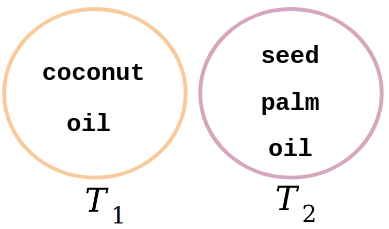
\includegraphics[width=1.0\textwidth]{imagenes/img1.png}
        \caption{Documentos representados como conjuntos}
    \end{subfigure}
    \hspace{5mm}
    \begin{subfigure}[b]{0.47\textwidth}
        \centering
        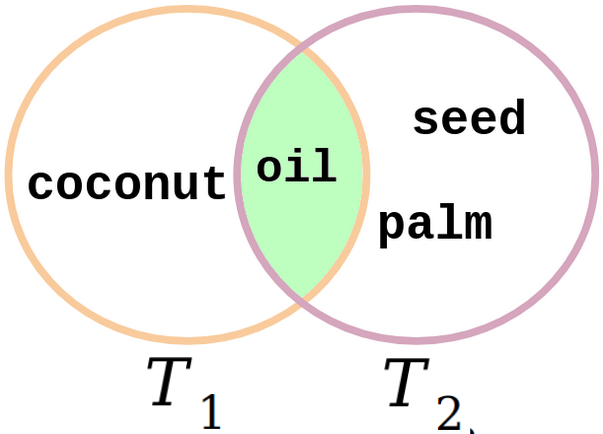
\includegraphics[width=0.80\textwidth]{imagenes/img5.png}
        \caption{Intersección entre los conjuntos de esos documentos}
    \end{subfigure}
    \caption{Intersección entre dos conjuntos}
    \label{fig:jaccard}
\end{figure}





\subsubsection{Distancia Levenshtein}
La distancia de Levenshtein es otra medida de concordancia entre descripciones textuales, y se define como el mínimo número de operaciones o movimientos que son necesarios para transformar una secuencia de caracteres en otra~\cite{yujian2007normalized}. Esta medida de distancia permite tanto trabajar de forma normalizada (por ejemplo, en el rango 0 a 1) como sin normalizar. 

Aplicada a nuestro problema en cuestión, hace referencia al número de movimientos necesarios para pasar de la descripción de un ingrediente a la de otro. Los movimientos permitidos vienen enumerados a continuación:

\begin{itemize}
    \item Eliminar un carácter: ABC $\xrightarrow{}$ AB, AC, BC
    \item Añadir un nuevo carácter: ABC $\xrightarrow{}$ ABCD, EABC, AEBC
    \item Sustituir un carácter por otro: ABC $\xrightarrow{}$ ABE, ADC, FBC
\end{itemize}


\subsection{Distancia semántica entre descripciones}

En este caso, se ha optado por una medida de distancia que utilice la representación numérica obtenida por el modelo de Word Embedding. Dado que esta representación se obtiene utilizando el contexto de cada palabra, trae de forma implícita la representación de su semántica. El utilizar medidas de distancia entre las representaciones numéricas de las palabras (o documentos) nos permitirá detectar si dos palabras son más o menos parecidas en función del contexto en el que se usen. 



\subsubsection{Distancia Word Mover's}

La medida de distancia Word Mover's trata los documentos cortos como representaciones de una nube de puntos, donde cada punto representa una palabra del documento expresada de forma vectorial a partir del modelo de Word Embedding. La distancia entre dos nubes se cuantifica como el coste que las palabras de un documento de texto deben asumir para coincidir exactamente con la nube de puntos del otro documento de texto~\cite{kusner2015word}. En nuestro caso, cada descripción alimenticia formará un documento corto.

\begin{figure}[H]
    \centering
    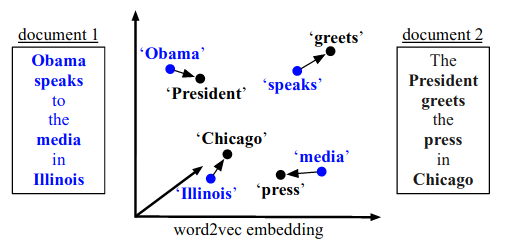
\includegraphics[width=0.7\textwidth]{imagenes/wmd.png}
    \caption{Funcionamiento de la distancia Word Mover's ~\cite{kusner2015word}}
    \label{fig:wmd}
\end{figure}

Para calcular la distancia entre dos palabras individuales, se utiliza una distancia euclídea entre las representaciones vectoriales correspondientes. De esta forma, se mantiene la semántica a la hora de obtener la similitud entre las palabras. En la Figura \ref{fig:wmd} se puede apreciar de manera gráfica el funcionamiento de esta medida de distancia. 

    
\subsection{Distancia híbrida entre descripciones}

En los apartados anteriores se han detallado medidas de distancias que tienen en cuenta la distancia entre descripciones desde un punto de vista puramente léxico o desde una aproximación basada en la semántica. 

Con el objetivo de obtener una mayor precisión en los resultados, se introduce una medida híbrida que tiene como objetivo combinar la capacidad sintáctica y la semántica de las descripciones textuales. Esta función de distancia se formula como una combinación ponderada de las distancias de Jaccard y Word Mover's (ver Fórmula~\ref{formula_hi}). Con esta medida, se pretende beneficiar aquellas descripciones textuales que sean similares desde un punto de vista sintáctico, sin olvidar la importancia de la semántica a la hora de alcanzar el resultado más preciso posible. 

    \begin{equation}
        HDISTANCE(t_{1},t_{2})=wJ(t_{1},t_{2}) + (1-w)WMD(t_{1},t_{2})
     \end{equation}
    \begin{center}
    donde $w\in {\rm I\!R}$ and $0 \leq w \leq 1$
    \end{center}\label{formula_hi}


\subsection{Fuzzificación de las medidas de distancia }
Cuando se trabaja con datos textuales, una de las cosas que hay que tener en cuenta es que hay que hacer frente a los problemas derivados de la ambigüedad del lenguaje. En capítulos anteriores ya se ha introducido la importancia de la semántica en el tratamiento de datos textuales. Esta importancia viene derivada de dificultades comunes que suelen aparecer al trabajar con información textual, como puede ser el uso de sinónimos, palabras muy similares, o incluso hacer frente a distintos niveles de detalle en las descripciones con las que trabajamos. 

Para lidiar con esta vaguedad existente en el lenguaje, se ha propuesto implementar medidas de distancia con Lógica Difusa que permitan dotar a nuestra herramienta de una mayor flexibilidad y robustez para hacer frente a este tipo de desafíos. En concreto, se han fuzzificado dos medidas de las detalladas en este capítulo, que se corresponden con Jaccard y Word's Mover. En ambas medidas se parte de la descripción textual como un conjunto de tokens, que se corresponden con la lista de palabras que forman la descripción textual a las cuales se les ha aplicado las tareas de preprocesamiento explicadas en el capítulo anterior. 



%The latter, along with the vagueness associated to the language (e.g., a mapping of two equivalent items with different level of specialization) calls for flexible approaches to calculate the mappings.

\subsubsection{Distancia difusa de Jaccard}
En este capítulo, se ha explicado el funcionamiento de la medida de distancia de Jaccard, la cual computa la distancia en base a la cantidad de elementos que forman parte de la intersección entre conjuntos. Dicha medida establece la intersección de forma estricta: un elemento pertenece al conjunto intersección solo si se encuentra de manera exacta en ambos conjuntos. Teniendo esto en cuenta, la medida de Jaccard no contempla que dos elementos similares se valoren a la hora de medir la similitud entre dos conjuntos.

Por la ambigüedad existente en el lenguaje y las múltiples formas de expresar una descripción alimenticia, se ha optado por implementar una versión difusa de la medida de Jaccard, que permita tener en cuenta el parecido entre los elementos de ambos conjuntos de manera proporcional al grado de similitud que tengan. De esta forma se valorará de forma positiva el parecido léxico entre los elementos que, sin llegar a formar parte de la propia intersección, sí tienen un grado de parecido notable que incita a ser considerados en el cálculo de la medida de distancia.

\begin{figure}[h!]
    \begin{subfigure}[b]{0.47\textwidth}
        \centering
        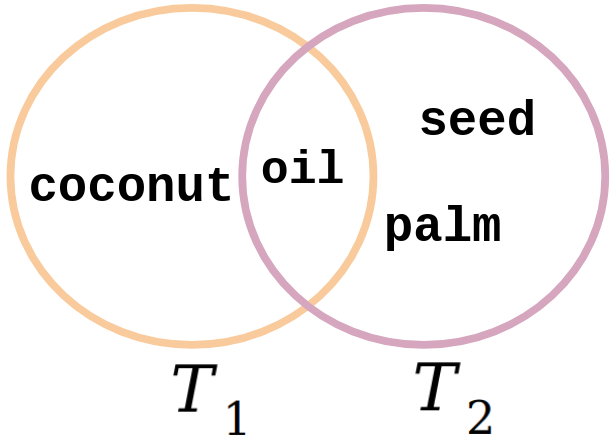
\includegraphics[width=0.8\textwidth]{imagenes/img2.png}
        \caption{Intersección clásica}
    \end{subfigure}
    \begin{subfigure}[b]{0.47\textwidth}
        \centering
        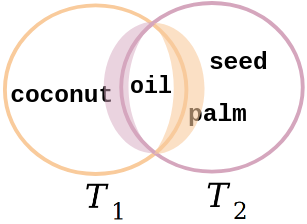
\includegraphics[width=0.78\textwidth]{imagenes/img3.png}
        \caption{Intersección difusa}
    \end{subfigure}
    \caption{Intersección entre dos conjuntos}
    \label{fig:jaccard_difuso}
\end{figure}

La versión difusa de Jaccard implementada se aprecia en la Fórmula \ref{formula:jaccard_fuz}~\cite{wang2011fast}. Consiste en una combinación de similitudes tanto a nivel de token como de carácter, con el objetivo de determinar el conjunto de intersección difusa que existe entre dos conjuntos (entendiendo cada descripción textual como un conjunto). Para conocer la distancia a nivel de token se utiliza la medida Jaccard que se ha descrito anteriormente, y mediante un umbral $\delta$ se determina cuáles de estos tokens forman parte del conjunto de intersección difuso. El valor del umbral se ha ajustado empíricamente al valor de 0.2. 

\begin{equation}
    \label{formula:jaccard_fuz}
    \tilde{J}_{\delta}(S_{1},S_{2})=\frac{\left | T_{1} \tilde{\cap}_{\delta} T_{2}\right |}{\left | T_{1} \right |+\left | T_{2} \right |-\left | T_{1}\tilde{\cap}_{\delta} T_{2} \right |}
\end{equation}
\begin{center}
    $\delta=0.2$
\end{center}

Para ilustrar el cálculo de esta medida, vamos a usar el mismo ejemplo que se empleó para la medida Jaccard (ver Figura \ref{fig:jaccard}) para ejemplificar cómo funciona su versión difusa. En la Figura \ref{fig:jaccard_difuso} se puede ver el valor de distancias a nivel de token entre ambos conjuntos.  Por simplificación, únicamente se muestran aquellas distancias cuyo valor es distinto de 1, y que por tanto, tienen alguna posibilidad de poder formar parte de la intersección difusa. En este caso, las líneas continuas, representan aquellos elementos cuya medida de distancia supera el umbral y por tanto se incluyen en la intersección difusa. Como se puede ver, en este caso el único elemento que lo supera es \texttt{oil}, por lo que la intersección tradicional y la difusa serían la misma: $J(S_{1},S_{2})=1-\frac{1}{2+3-1} = 0.75$.

\begin{figure}[H]
    \centering
    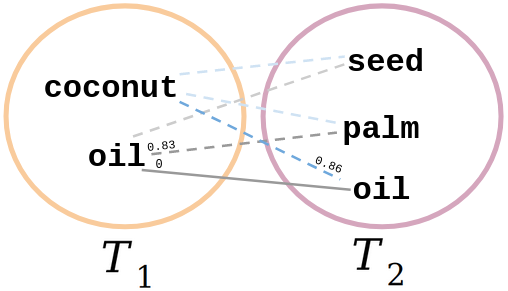
\includegraphics[width=0.7\textwidth]{imagenes/img4.png}
    \caption{Función de distancia difusa Jaccard}
    \label{fig:fuzzy_jaccard_metric}
\end{figure}


Ahora imaginemos que, en un hipotético caso, la distancia entre \textit{coconut} y \textit{palm} es 0.1 porque son extremadamente similares, y por tanto entraría dentro del conjunto de la intersección difusa al no superar el umbral. Si aplicamos la fórmula de la distancia difusa de Jaccard, se quedaría tal que $J(S_{1},S_{2})=1-\frac{1+0.9}{2+3-1-0.9} = 0.39$, un valor inferior que el obtenido con la versión clásica, que sí representaría esta valoraría la similitud entre los elementos.

\subsubsection{Distancia difusa entre documentos}
Se ha diseñado una medida de la distancia entre documentos cortos partiendo de un enfoque difuso, considerando cada documento como el conjunto de tokens que se obtienen del preprocesamiento de la descripción textual.

En las medidas que trabajan con conjuntos que se han utilizado hasta ahora, (entre ellas incluida la medida difusa de Jaccard) se hace hincapié en el parecido de los elementos entre conjuntos uno a uno. Sin embargo, parece interesante medir la distancia de un elemento a un conjunto completo, en lugar de distancia entre elemento y elemento. Esto permitiría obtener una medida que valore el papel de cada elemento al nivel de la descripción textual, y no elemento a elemento lo cual podría resultar poco apropiado, puesto que no se estaría teniendo en cuenta a la descripción como un todo. Por ello, se ha propuesto en este trabajo la medida de distancia $\tilde{D}$, la cual se centra en esta afirmación y cuyo cálculo se expone en la Fórmula \ref{formula:fuzzy-document}. Para poder obtener el valor de distancia $\tilde{D}$ entre las descripciones textuales $S_{1}$ y $S_{2}$ se tienen en cuenta los siguientes puntos:

\begin{enumerate}
    \item Obtener el conjunto unión ($T_{1}\cup T_{2}$) de los conjuntos $T_{1}$ y $T_{2}$ , los cuales se corresponden respectivamente con el conjunto de tokens que forman las descripciones $S_{1}$ y $S_{2}$. %AÑADIR EJEMPLOS
    
    \item Calcular, para cada elemento presente en los conjuntos $T_{1}$ y $T_{2}$ (el cual se encuentra en el conjunto $T_{1}\cup T_{2}$) su grado de pertenencia al conjunto contrario. Para calcular el grado de pertenencia de un elemento a un conjunto, se utiliza la función $\mu_{T_{i}}(x)$, donde $i$ hace referencia al conjunto y $x$ al elemento del que se quiere obtener el grado de pertenencia a dicho conjunto $i$.
    

    \item Calcular el valor de la intersección difusa de los dos conjuntos. Para calcular el grado de pertenencia de un elemento a un conjunto, se utiliza la función $\mu_{T_{i}}(x)$ comentada en el punto anterior.
    \item El valor de distancia se corresponde con el resultado de la sumatoria en el paso 2 dividido entre el valor de la intersección en el paso 3.
\end{enumerate}

Como se puede apreciar en el cálculo de dicha medida, se hace uso de la función de pertenencia $\mu_{T_{i}}(x)$ la cual permite obtener el grado de pertenencia del elemento $x$ al conjunto $T_{i}$, donde $x$ hace referencia a un elemento de un conjunto obtenido a partir de una descripción textual, y  $T_{i}$ es el conjunto que representa a la descripción textual $S_{i}$.

\begin{equation}
\label{formula:fuzzy-document}
   \textstyle \tilde{D}(S_{1},S_{2})=\frac{\sum_{x\epsilon T_{1}\cup T_{2} }min(\mu T_{1})x \times min(\mu T_{2})x}{\sum_{x\epsilon T_{1} }(\mu T_{1} )(x)+\sum_{x\epsilon T_{2} }(\mu T_{2} )(x)-\sum_{x\epsilon T_{1}\cup T_{2} }min(\mu T_{1})x \times min(\mu T_{2})x}  
\end{equation}\label{for:pertenencia}
    

\begin{equation}
\label{formula:fuzzy-document-2}
\mu_{T_{i}}(x)= \left\{ \begin{array}{lcc}
         1 &   & d_{E}(t_{i},x) = 0 \\
         \\ 0 &   &  d_{E}(t_{i},x) = \infty \\
         \\ sigmoid(\frac{1}{d_{E}(t_{i},x)}) &    & 0 < d_{E}(t_{i},x) < \infty 
         \end{array}
\right .   
\end{equation}
\begin{center}
    donde $d_{E}(t_{i},x)$ es la distancia euclídea entre $t_{i}$ y $x$
\end{center}
    
En la práctica, al determinar el grado de pertenencia de un elemento a un conjunto, estamos haciendo referencia al parecido entre los elementos de descripciones. Para ello, se ha diseñado una función de pertenencia, la cual se puede observar en la fórmula Fórmula \ref{for:pertenencia}. Para la definición de esta función, En primer lugar hay que determinar la medida de distancia entre dos elementos textuales procedentes de descripciones. En este caso, la distancia entre dos elementos o tokens procedentes de las  descripciones se calcula como la distancia euclídea entre los vectores de los tokens de ambos conjuntos. Estos vectores corresponden a la representación numérica obtenida del modelo de Word Embedding previamente entrenado. En función del resultado que se obtenga con la distancia euclídea, se consideran tres casuísticas, las cuales se contemplan en la función de pertenencia:

\begin{enumerate}
    \item Si el valor de distancia euclídea entre los vectores de dos palabras del vocabulario es 0, las dos palabras son idénticas, por lo que el grado de pertenencia es máximo. En nuestro caso, este valor es 1 y representa la máxima similitud. Esta situación se encuentra contemplada en el primer caso de la función de pertenencia (ver fórmula \ref{formula:fuzzy-document}).
    
    \item El segundo caso contemplado en la función de pertenencia (ver fórmula \ref{formula:fuzzy-document}) hace referencia a aquellas situaciones donde el valor de distancia euclídea sea $\infty$. Que se obtenga dicho valor significa que no se ha podido determinar la distancia entre elementos porque no se tiene representación vectorial de alguno de ellos, o incluso de ambos. En este caso al no poder determinarse un valor de distancia, no hay pertenencia posible y como resultado, el grado de pertenencia es 0, que representa similitud nula.
    
    \item Si el valor de distancia euclídea se encuentra en el intervalo $(0,\infty)$, estamos en el último caso contemplado por la función de pertenencia. Puesto que estamos trabajando con grados de pertenencia, para poder acotar el problema debemos trasladar este valor de distancia al intervalo (0,1). Para ello, se ha utilizado el valor de la función \textit{sigmoide} de la inversa de la distancia. Con este cálculo, conseguimos trabajar con valores acotados en el intervalo (0,1) que representen la similitud entre dos elementos. 
\end{enumerate}


Con esta medida, se premia a aquellos elementos que aparecen en ambos conjuntos, a la vez que se combina con el parecido existente entre los tokens que no forman parte de la intersección. Además, con la función de pertenencia utilizada se tiene en cuenta la carga semántica que contempla el modelo de Word Embedding descrito en la sección anterior, dotando así de una mayor flexibilidad a la herramienta. 

\section{Elección de la medida de distancia}

Para analizar el funcionamiento de este módulo y evaluar la calidad de los resultados obtenidos con las distintas métricas, se ha estudiado el comportamiento de cada una de las medidas expuestas en la sección anterior aplicando este módulo a un problema de mapeo de datos entre dos bases de datos de composición nutricional, detallado en el Capítulo \ref{ch:Pruebas}. El objetivo de esta tarea de mapeo de datos es estudiar cómo se comportan las distintas medidas de distancia utilizadas, y poder concluir cuál de ellas se adapta mejor al problema y es capaz de identificar elementos equivalentes con mayor precisión. 
